\documentclass[aps,prd,twocolumn,10pt,nofootinbib,superscriptaddress,floatfix]{revtex4-2}
\usepackage{amsmath,amssymb,bm,graphicx,booktabs}
\usepackage[colorlinks=true,allcolors=blue]{hyperref}
\newcommand{\ii}{\mathrm{i}}
\newcommand{\dd}{\mathrm{d}}
\begin{document}
\title{Enhanced nonlinear phase response at flux-response zeros in near-extremal Kerr scattering}
\author{Jing-Qi Lai}
\email{laijingqi19@mails.ucas.ac.cn}
\affiliation{School of Physical Sciences, University of Chinese Academy of Sciences, Beijing 100049, China}
\author{Yu Tian}
\email[Corresponding author: ]{ytian@ucas.ac.cn}
\affiliation{School of Physical Sciences, University of Chinese Academy of Sciences, Beijing 100049, China}
\affiliation{Institute of Theoretical Physics, Chinese Academy of Sciences, Beijing 100190, China}
\date{Research draft, October 17, 2026}
\begin{abstract}
We study the complex first-order transmission response of a massless,
self-interacting scalar field on a fixed near-extremal Kerr background.
An exact Green-function decomposition separates the energy-flux response
from the transmitted phase response. For the interaction $|\Phi|^6\Phi$,
spectral calculations at $a/M=0.999999$ and $(\ell,m)=(2,2)$ resolve a
simple flux-response zero near $(\omega-m\Omega_H)/\kappa=2.41954$,
with a dimensionless phase-response coefficient of approximately $10316$.
Leading near-extremal matching predicts a nearby zero at $2.42349$.
Principal modes yield a complex response with a $\sigma^{-n}$ envelope
and logarithmic modulation, where $\sigma=(r_+-r_-)/M$.
This draft assembles the established first-order identities, existing
numerical evidence, and specific tests of zero curves, finite-coupling
fluxes, and wave-packet observables required for a broader interpretation.
\end{abstract}
\maketitle

\section{Question and scope}
The question is whether an enhanced complex nonlinear scattering response
can have a vanishing first-order energy-flux projection at selected real
frequencies. We consider a prescribed Kerr metric, a complex scalar field,
and stationary illumination from infinity. Linear near-extremal scattering
and critical behavior provide the matching framework
\cite{Bredberg,GrallaTransient,GrallaCritical}.
Weakly nonlinear gravitational mode dynamics has a different field equation
and initial-value formulation \cite{Weather}.
The present evidence concerns the derivative at zero scalar coupling.
The status of finite-coupling observables is specified in Sec.~\ref{sec:next}.

\section{Conventions and response coefficients}
We use $G=c=1$, signature $(-,+,+,+)$, and Fourier dependence
$e^{-\ii\omega t+\ii m\phi}$. Define
\begin{gather}
\Delta=(r-r_+)(r-r_-),\quad r_\pm=M\pm\sqrt{M^2-a^2},\\
\frac{\dd r_*}{\dd r}=\frac{r^2+a^2}{\Delta},\quad
\Omega_H=\frac{a}{r_+^2+a^2},\quad
\kappa=\frac{r_+-r_-}{2(r_+^2+a^2)},\\
p=\omega-m\Omega_H,\quad y=p/\kappa,\quad
\sigma=(r_+-r_-)/M.
\end{gather}
For $\Box\Phi+\epsilon_n|\Phi|^{2n}\Phi=0$, let
$g_n=\epsilon_n/M^{2n-2}$ and
$\eta=g_n|\mathcal A_{\rm in}|^{2n}$, with the incident normalization
held fixed. In the incident angular channel,
\begin{align}
C_H&=C_H^{(0)}[1+\eta\rho_n+O(\eta^2)],\\
T/T^{(0)}&=1+\eta\chi_n+O(\eta^2),\\
\Delta\arg C_H&=\eta\psi_n+O(\eta^2),\quad
\chi_n=2\Re\rho_n,\quad\psi_n=\Im\rho_n.
\end{align}
The coefficients $T$ and $R$ denote signed horizon and outward infinity
energy fluxes divided by the incident energy flux. Orthogonality of the
normalized spheroidal harmonics selects the incident angular channel in
the integrated first-order interference flux. Additional angular channels
enter the flux at second order in the coupling.

\section{Exact flux--phase decomposition}
For real $\omega$, choose a unit-ingoing-horizon solution $R_{\rm in}$
and a unit-outgoing-infinity solution $R_{\rm up}$:
\begin{align}
R_{\rm in}&\sim e^{-\ii p r_*}\quad(r\to r_+),\\
R_{\rm in}&=B^{\rm inc}R_{\rm up}^*+B^{\rm ref}R_{\rm up},\\
R_{\rm up}&\sim r^{-1}e^{\ii\omega r_*}\quad(r\to\infty).
\end{align}
The radial operator is
\begin{equation}
\mathcal L R=(\Delta R')'+(K^2/\Delta-\lambda)R,
\quad K=(r^2+a^2)\omega-am.
\end{equation}
With $\int |S|^2\dd\Omega=1$, define
\begin{equation}
C_j^{(n)}=\int (\cos\theta)^j|S|^{2n+2}\dd\Omega,\quad
P_n=r^2C_0^{(n)}+a^2 C_2^{(n)}.
\end{equation}
The self-channel sourced equation has
$\mathcal L R_1=-P_n|R_{\rm in}|^{2n}R_{\rm in}$ in the
unit-horizon normalization. Its Wronskian is
$W=\Delta(R_{\rm in}R_{\rm up}'-R_{\rm up}R_{\rm in}')
=2\ii\omega B^{\rm inc}$.
Writing $q=B^{\rm ref}/B^{\rm inc}$ gives
\begin{align}
J_{d,n}&=\int_{r_+}^{\infty}P_n|R_{\rm in}|^{2n}|R_{\rm up}|^2\dd r,
\\
J_{o,n}&=\int_{r_+}^{\infty}P_n|R_{\rm in}|^{2n}R_{\rm up}^2\dd r,
\\
\rho_n&=\frac{\ii M^{2n-2}}{2\omega|B^{\rm inc}|^{2n}}
(J_{d,n}+qJ_{o,n}).
\end{align}
Since $J_{d,n}$ is real,
\begin{align}
\chi_n&=-\frac{M^{2n-2}\Im(qJ_{o,n})}{\omega|B^{\rm inc}|^{2n}},\\
\psi_n&=\frac{M^{2n-2}[J_{d,n}+\Re(qJ_{o,n})]}
{2\omega|B^{\rm inc}|^{2n}}.
\end{align}
Thus $\Im(qJ_{o,n})=0$ is the flux-zero condition. The direct real
integral remains active in the phase. At such a zero the first-order
transmitted amplitude is tangent to the constant-modulus circle.

\section{Principal-mode enhancement and zeros}
At fixed $y$, principal modes have $h=1/2+\ii\beta$.
The equal real exponents of the two matching branches give
$|B^{\rm inc}|^{-2}\sim\sigma^{-1}|\mathcal D|^{-2}$.
The leading throat Green integral is convergent for the interaction powers
considered here. Combining its finite unit-horizon coefficient with the
incident normalization gives
\begin{equation}
\rho_n=\sigma^{-n}\mathcal G_n(y,\beta\ln\sigma)
+o(\sigma^{-n}).
\end{equation}
The leading coefficient has period $\pi$ in its second argument.
For $(2,2)$, $\beta\simeq0.94595847$ and
$\Delta\ln\sigma=\pi/\beta\simeq3.32107$.
The leading zero condition is $\Re\mathcal G_n(y_\star,\beta\ln\sigma)=0$.
For a simple zero its local drift obeys
\begin{equation}
\frac{\dd y_\star}{\dd\ln\sigma}
=-\beta\frac{\partial_\theta\Re\mathcal G_n}
{\partial_y\Re\mathcal G_n},\quad\theta=\beta\ln\sigma.
\end{equation}
Finite-$\sigma$ corrections shift this leading curve. Tracking the curve
through a complete logarithmic period is a proposed numerical test.

\section{Numerical evidence}
The endpoint-inclusive Chebyshev solver enforces the regular-singular
horizon relation and the peeled-field normalization at the horizon.
The Green integrals use Gauss integration on panels uniform in
$\ln[(r-r_+)/(r_+-r_-)]$, with an analytic endpoint contribution.
Existing refinements cover 81 principal-mode parameter points with
$(\ell,m)=(2,2),(3,3),(4,4)$, $n=1,2,3$, $y=-0.5,0.5,1$,
and $a/M=0.9999,0.99999,0.999999$.
The largest paired change in the real response is $6.55\times10^{-9}$;
this is an order-refinement diagnostic. Separate residual and flux tests
measure the field and balance errors.
The phase-focused scan contains 27 parameter points for $(2,2)$.
\begin{table}[b]
\caption{Full Kerr responses at $M=1$, $a=0.999999$, $(\ell,m)=(2,2)$,
and $n=3$. The physical corrections include the factor $\eta$.}
\begin{ruledtabular}
\begin{tabular}{ccc}
$y$&$\chi_3$&$\psi_3$\\
2&363.069&24131.5\\
2.41954&$\simeq0$&10316.0\\
4&$-0.0102804$&1571.09
\end{tabular}
\end{ruledtabular}
\end{table}
The signed root bracket is $[2.41934036,2.41974036]$.
At its ends $\chi_3\simeq0.0113165$ and $-0.0112885$.
Checks with spectral orders 448 and 576, integration orders 48 and 64,
and matching radii 8, 12, and 16 give
$|\chi_3|\leq5.73\times10^{-9}$ at the common root estimate.
The independently reconstructed sourced field has a best tested
off-grid relative residual of $9.10\times10^{-9}$ on
$(r-r_+)/(r_+-r_-)\in[1,8]$; higher reconstruction orders expose a
numerical floor. The relative residual denominator includes the field
in every operator term.
\begin{figure*}
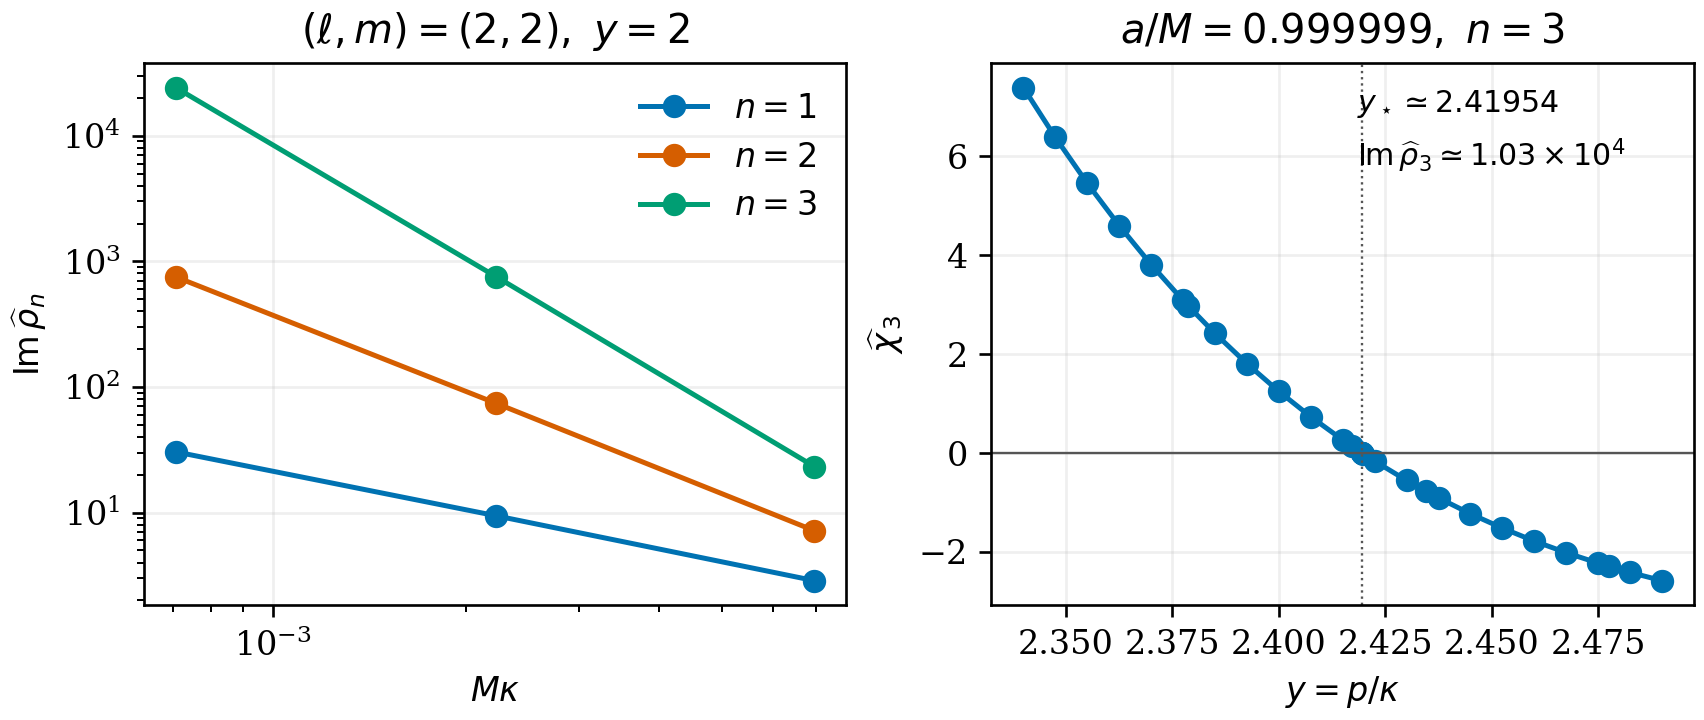
\includegraphics[width=0.95\textwidth]{../../figures/kerr_scalar_phase_flux_separation_20261014.png}
\caption{Existing spectral results for the enhanced phase coefficient
and the resolved flux-response zero. The phase scan and the zero scan
use their indicated parameter slices.}
\end{figure*}
Leading matching at the numerical zero predicts $\psi_3\simeq10360.0$,
a difference of about $0.43\%$ from the full Kerr value.
It predicts $\chi_3\simeq0.2222$ there. Solving the leading matched
zero condition gives $y_\star\simeq2.42349$, shifted by approximately
$0.00395$ from the Kerr root. The analytic construction therefore
captures a nearby zero and the phase scale, with finite-$\sigma$
corrections required for the root location.

\section{Open tests and interpretation}\label{sec:next}
The current result establishes a stable first-order flux zero in one
principal-mode, interaction-power, and spin slice.
Further work will trace zeros versus spin, detuning, mode, and interaction
power, and compute the next matching correction.
At fixed $y=2$ the phase coefficients for $n=1,2,3$ show increasing
near-extremal enhancement. Establishing a general zero family requires
additional signed brackets and refinement tests in each slice.

For a transmission expansion $C/C_0=1+\eta\rho_1+\eta^2\rho_2+\cdots$,
the second-order flux coefficient is
\begin{equation}
|\rho_1|^2+2\Re\rho_2.
\end{equation}
The second-order sourced field and additional angular-channel fluxes
are required to determine the finite-coupling energy response.
The horizon perturbative condition is $|\eta\rho_n|\ll1$;
global field control also requires spatial and angular checks.

External phase observables require the reflected amplitude or a
finite-bandwidth wave packet. Under a conditional duration estimate
$\tau\propto\kappa^{-1}$ and fixed incident energy, the incident
power scales as $\kappa$ and can compensate the stationary
$\kappa^{-n}$ enhancement. A quantitative packet prediction requires
the frequency convolutions in $|\Phi|^{2n}\Phi$.
These tests define the observable interpretation and the range of a
possible short-paper claim.

\appendix
\section{Evidence and reproduction}
The existing numerical records are dated October 14, 2026:
\texttt{kerr\_scalar\_letter\_refinement},
\texttt{kerr\_scalar\_phase\_dominance}, and
\texttt{kerr\_scalar\_flux\_zero}, including the sourced-field checks.
The archive contains the corresponding CSV and JSON files.
The leading matching root quoted here was evaluated from
\texttt{near\_data}, \texttt{integrals}, and \texttt{coefficients}
in the existing principal-matching scripts, with 20-point Gauss panels
over logarithmic near-coordinate limits $[-36,36]$ and Brent root finding.
The matching result is an asymptotic prediction in the current draft.

\begin{thebibliography}{9}
\bibitem{Bredberg} I. Bredberg, T. Hartman, W. Song, and A. Strominger,
Black hole superradiance from Kerr/CFT, JHEP \textbf{04} (2010) 019,
doi:10.1007/JHEP04(2010)019, arXiv:0907.3477.
\bibitem{GrallaTransient} S. E. Gralla, A. Zimmerman, and P. Zimmerman,
Transient instability of rapidly rotating black holes,
Phys. Rev. D \textbf{94}, 084017 (2016), doi:10.1103/PhysRevD.94.084017.
\bibitem{GrallaCritical} S. E. Gralla and P. Zimmerman,
Critical exponents of extremal Kerr perturbations,
Class. Quantum Grav. \textbf{35}, 095002 (2018), doi:10.1088/1361-6382/aab140.
\bibitem{Weather} C. Iuliano, S. Hollands, S. R. Green, and P. Zimmerman,
Extremal black hole weather, Phys. Rev. D \textbf{111}, 124038 (2025),
doi:10.1103/PhysRevD.111.124038.
\end{thebibliography}
\end{document}
